\chapter{提案手法と実験概要}  
本章では,本研究が最終的に目指す津波避難誘導問題への解決策として,マルチエージェント強化学習と自律飛行型ドローンを組み合わせた提案手法について述べる.
また,提案手法が既存研究と異なる点や新規性についても論じる.

\section{提案手法の概要} 
\label{sec:sug} 
本研究では,観光地や都市部といった地元住民以外にも多数の人々が屋外に存在する状況を想定している.
これには,日常的に避難訓練を受けていない観光客や土地勘のない訪問者も含まれる.
このような状況や,前章で述べた避難誘導における課題を背景に,地震発生後の津波避難という非常に緊急性の高い場面を想定し,避難誘導を行うための手法を検討する.
従来,自治体職員や警察・消防隊員といった人間が担ってきた避難誘導を,自律飛行型ドローンが代替するシステムを構築することを目標とする.

具体的には,マルチエージェント強化学習を活用し,複数のドローンエージェントが協調して行動する能力を学習させることで,刻々と変化する被災地域の状況を動的に認識し,群衆の避難完了率を最大化することを目指す.
また,避難者の位置,避難経路上の障害物,各ドローンの位置などをリアルタイムに反映するデジタルツイン環境を構築し,その環境内で学習済みのエージェントがシミュレーションを通じて最適な誘導方法を実行できるようにする.
さらに,デジタルツイン環境と実機ドローンを連動させることで,現実世界での運用を可能とする動的な避難誘導システムを構築する.

\begin{figure}[H] 
  \centering 
  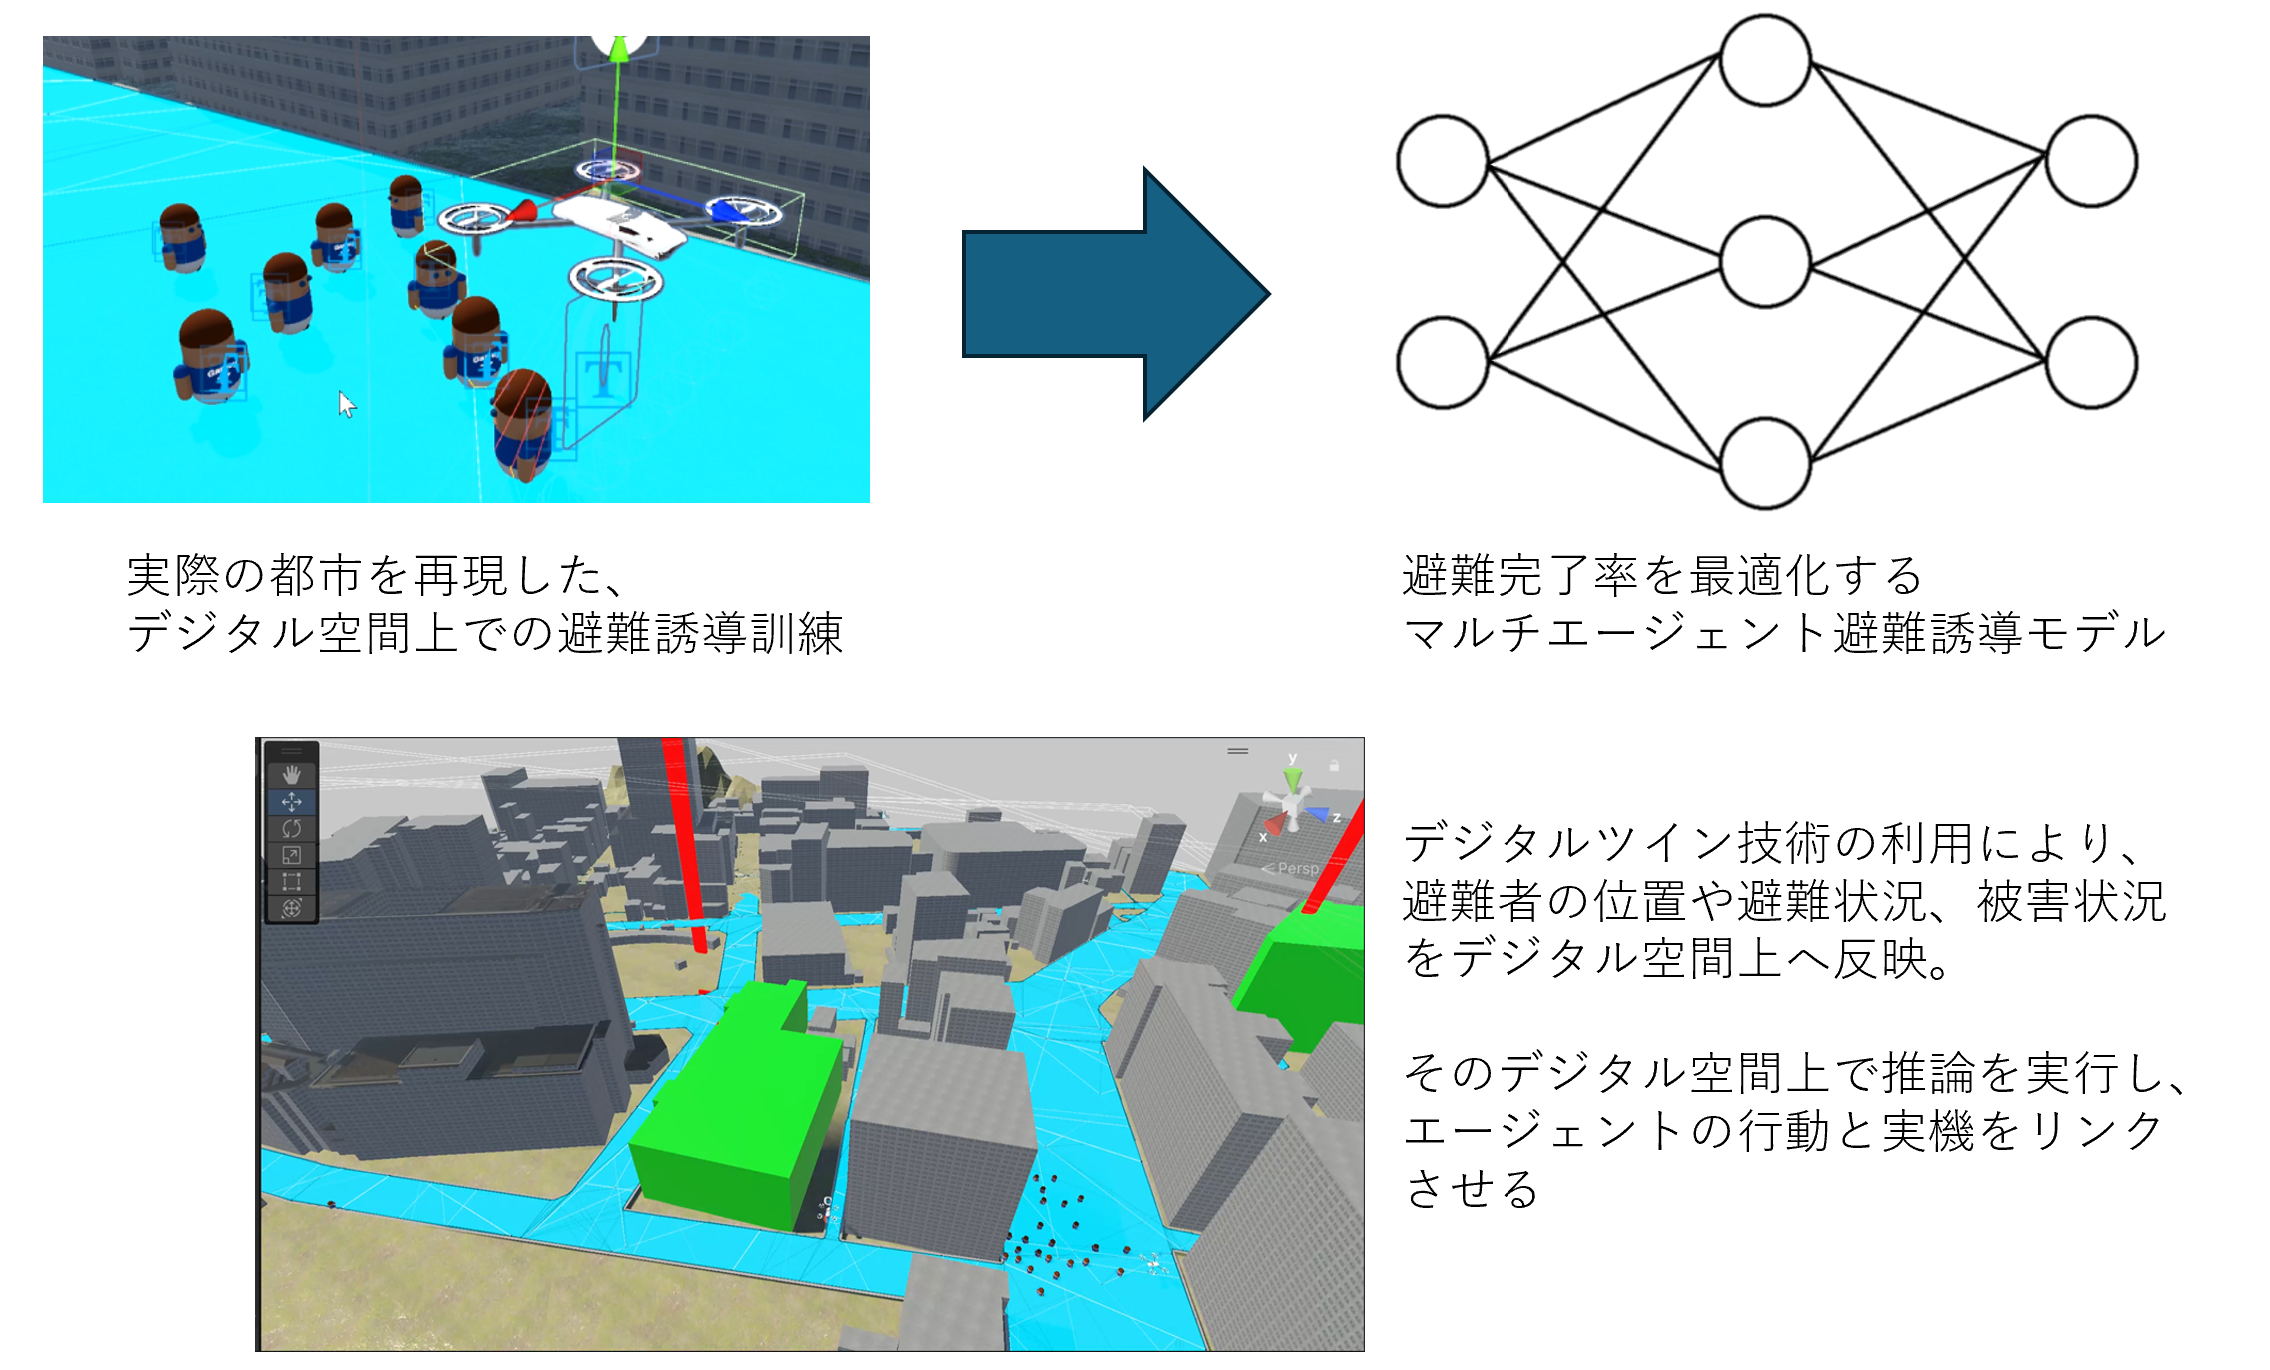
\includegraphics[width=1.0\textwidth]{Figures/2024-12-06 182816.png}
  \caption{提案手法 概略図} 
  \label{fig:01} 
\end{figure}

\section{既存研究との新規性}  
研究背景で述べたとおり,本研究は既存の研究といくつかの重要な相違点や新規性を有している.

まず,ドローンの防災活用はまだ研究が始まったばかりの新しい分野であり,本研究はその発展に寄与するものである.特に,複数のドローンを連携して運用するシステムに,AIや強化学習モデルを導入する点は,本研究の独自性を示す重要な要素である.

さらに,本研究では都市モデルを活用した訓練環境を構築し,デジタルツイン技術を通じて現実環境における運用を想定している.このように,現実世界での実用性を考慮した研究は,防災分野においても新しい試みである.

また,本研究は避難ビルの収容定員など,経路条件以外の要素を考慮した避難誘導モデルの作成にも取り組んでいる.
従来の研究の多くが,避難者自身の行動最適化を通じて避難完了率の向上を目指しているのに対し,本研究では避難完了率を最適化できる避難誘導方策そのものを追求している点で特徴的である.

以上のような取り組みにより,本研究は現実世界での応用可能性を持つ動的な津波避難誘導システムの実現を目指している.


\section{シミュレーション・学習環境構築}
\subsection{環境全般}
\subsection{都市モデルの選定と避難所の配置条件}
環境としては,下記3つの都市の都市モデルをPLATEAU SDK for Unityを使い実際の都市環境に近いシミュレーション環境を再現する.
なお,都市の選定基準については,\ref{sec:sug}章にて述べた想定場面を考慮するため下記の選定基準をもって決定した.
\begin{enumerate}
  \item 南海トラフ等で津波被害が想定されている沿岸地域であること
  \item 自治体の津波避難のハザードマップが参照可能であること
  \item 地元住民以外にも多数の観光客が見込まれる,比較的規模の大きな地域であること
  \item 津波避難ビルあるいは津波避難タワーが整備されている地域であること
\end{enumerate}
以上の条件を元に,下記3つの都市をモデル都市として選択した.
\begin{enumerate}
  \item 神奈川県横須賀市 市役所周辺沿岸地域
  \item 静岡県沼津市 沼津港周辺の一部地域
  \item %% TODO;追加実験
\end{enumerate}
都市モデルと実際の避難ビル(避難タワー)との位置付けは,自治体公表のハザードマップより目算により算出し,都市モデル上で指定した.
各モデル都市におけるシミュレーション対象範囲は下図の通りである.
% TODO : シミュレーション範囲図の添付

\subsection{避難者の行動設計}
本環境で使用する避難者の行動モデルは下図のフロー通りとなる.
\begin{figure}[H] 
  \centering 
  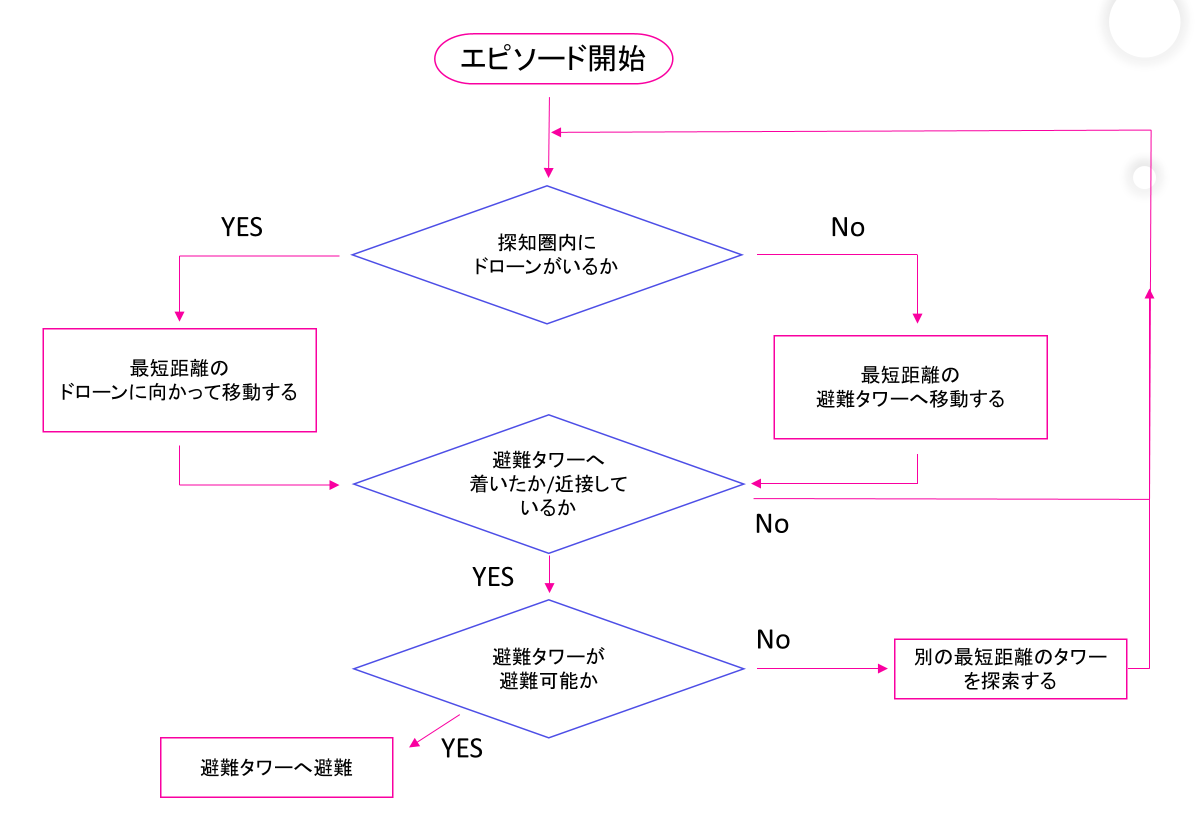
\includegraphics[width=1.0\textwidth]{Figures/334170449-c22ed682-06c1-4fbc-ba4b-07d946d8a047.png}
  \caption{避難者の行動フロー} 
  \label{fig:01} 
\end{figure}


\section{エージェントモデル}
  \subsection{移動経路の計算方法}
  \subsection{観測情報}
  \subsection{報酬関数と行動評価}


\section{実験概要}
  \subsection{誘導タスクにおける比較実験}
